\appendix
%
% ***
\chapter{UML-Diagramme wichtiger Algorithmen}
\label{app:UML}
% ***
%

	% ***
	\section{\texttt{RandomSearch}}
	\label{app:UML_RS}
	% ***
		Die folgende Abbildung \ref{fig:uml_rs} stellt den genutzten Algorithmus \texttt{RandomSearch} qualitativ in einem Programmablaufplan vor.
		\begin{figure}[H]
			\centering
			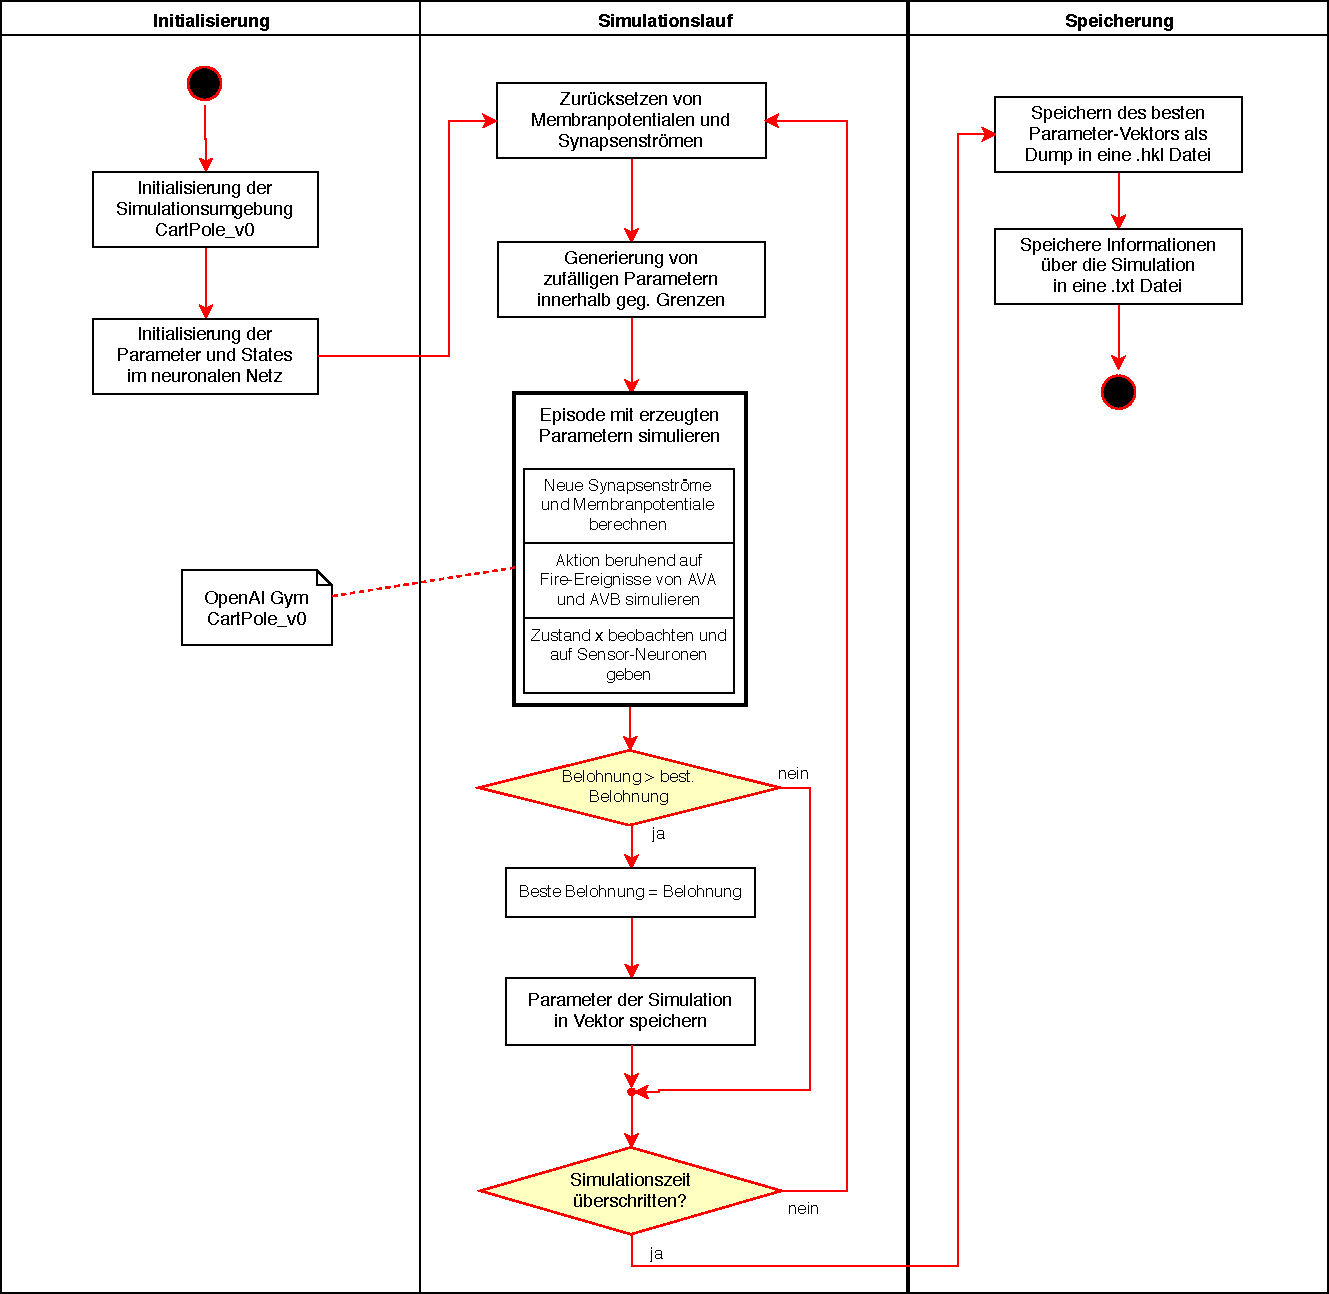
\includegraphics[width=14cm]{figures/appendix/uml_rs.pdf}
			\caption{UML Diagramm des Algorithmus \texttt{RandomSearch}.}
			\label{fig:uml_rs}
		\end{figure}
	
	% ***
	\section{\texttt{Weights}}
	\label{app:UML_RS}
	% ***
	Die folgende Abbildung \ref{fig:uml_weights} stellt den genutzten Algorithmus \texttt{Weights} qualitativ in einem Programmablaufplan vor.
	\begin{figure}[H]
		\centering
		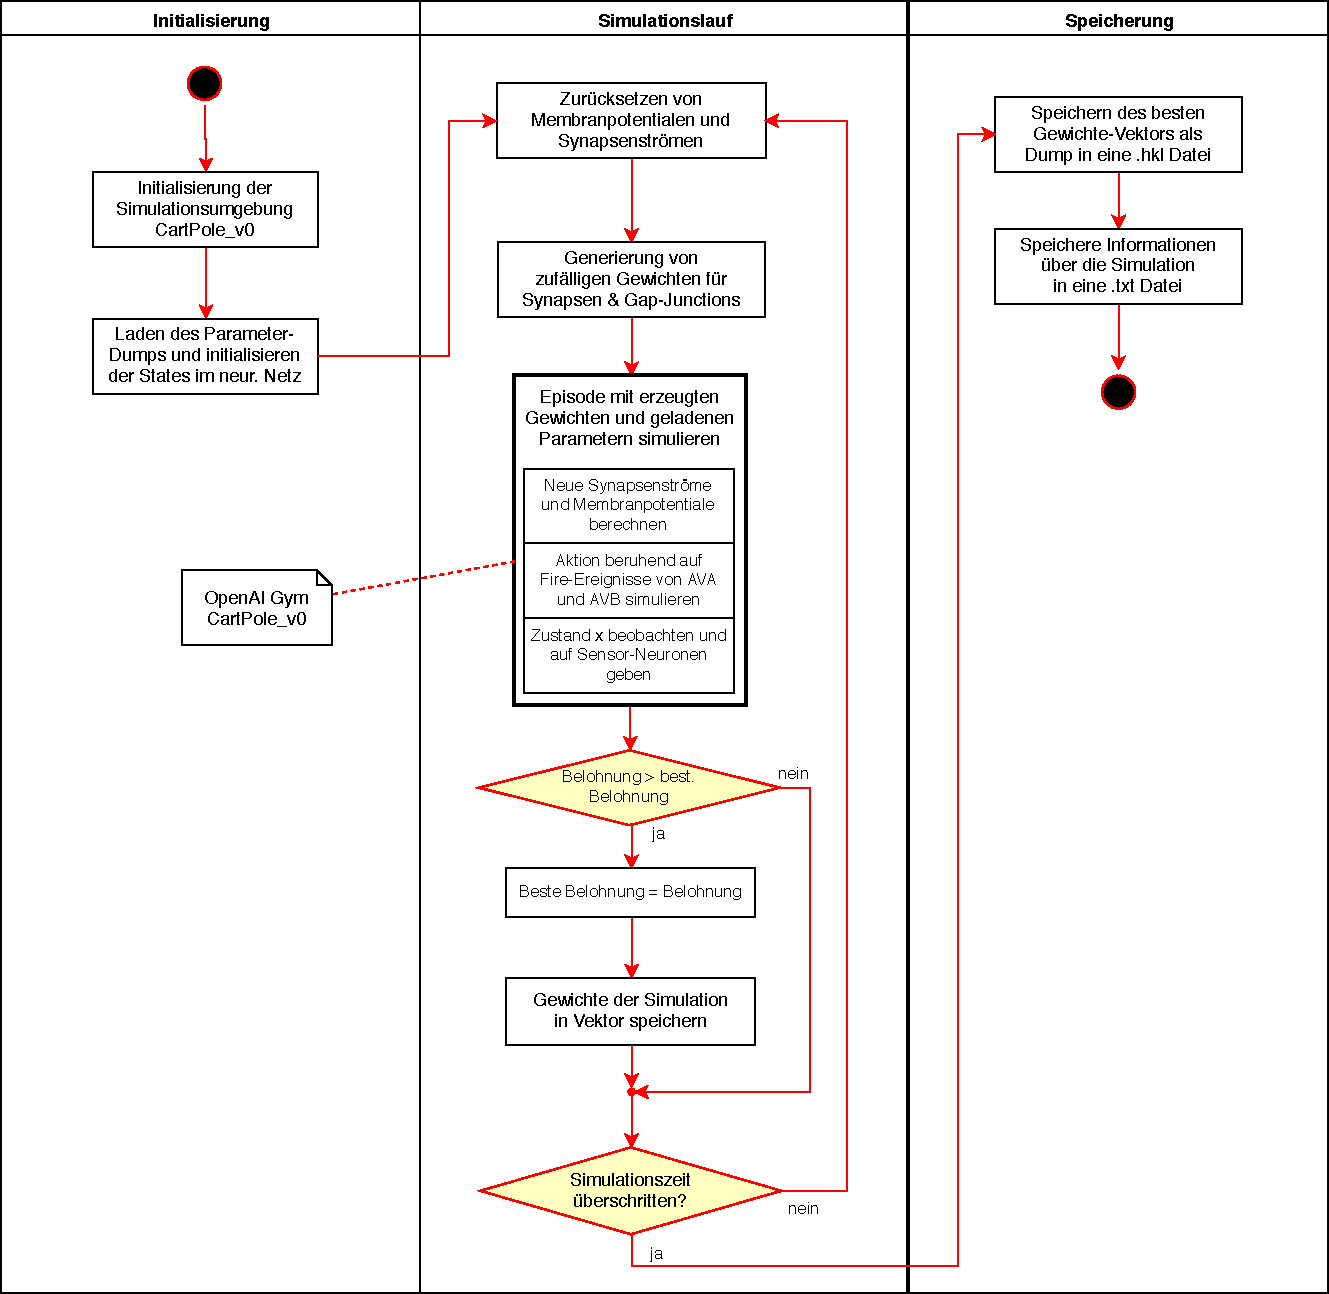
\includegraphics[width=14cm]{figures/appendix/uml_w.pdf}
		\caption{UML Diagramm des Algorithmus \texttt{Weights}.}
		\label{fig:uml_weights}
	\end{figure}

%
% ***
\chapter{Datenblatt Programm: TW Circuit}
% ***
%
\label{app:datenblatt}
\enlargethispage{2\baselineskip}
\begin{minipage}[b]{0.61\textwidth}
	\begin{mybox}{Name}
		\texttt{TW Circuit}
	\end{mybox}
	\begin{mybox}{Kurzinfo}
		\texttt{Das Programm TW Circuit dient als Simulator des Touch Withdrawal Circuit des Wurms \textit{C. Elegans} \cite{WormLevelRL}. Es kann ein beliebig aufgebautes, neuronales Netz mit biologischem Hintergrund implementiert werden. Dazu wird das LIF - Modell genutzt, um die neuronale Dynamik zu simulieren und Feuer-Events vorherzusagen. Der Output wird auf eine beliebige Simulationsumgebung gegeben, in diesem Beispiel wird OpenAI's CartPole\_v0 genutzt.\\ Der Simulator ist OpenSource und kann beliebig erweitert oder verändert werden. Er verfügt darüber hinaus auch über Inspektionsfunktionen sowie gut dokumentierten Code, um Befehle schnell nachzuvollziehen.}
	\end{mybox}
	\begin{mybox}{Dependencies}
		\begin{itemize}
			\item \texttt{NumPy} aus dem \texttt{SciPy}-Package
			\subitem Numerische Berechnungen und Matrixoperationen.
			\item \texttt{matplotlib} aus dem \texttt{SciPy}-Package
			\subitem Plots und Grafiken anzeigen und exportieren.
			\item OpenAI Gym
			\subitem Simulationsumgebung \texttt{CartPole\_v0}
			\item \texttt{hickle}
			\subitem Performantes Speichern im HDF5-Format
			\item \texttt{os, time, datetime}
		\end{itemize}
	\end{mybox}
\end{minipage}
%\hfill
\begin{minipage}[b]{0.38\textwidth}
	\begin{mybox}{QR-Code}
		\centering
		
\includegraphics[width=0.9\textwidth]{figures/appendix/qr-code.pdf}
	\end{mybox}
	\begin{mybox}{Dateibaum}
		\vspace{0.1cm}
		\begin{forest}
			pic dir tree,
			where level=0{}{% folder icons by default; override using file for file icons
				directory,
			},
			[TW Circuit
			[docs]
			[information]
			[modules
			[genetic\_algorithm.py, file]
			[inspect.py, file]
			[lif.py, file]
			[parameters.py, file]
			[random\_search\_v2.py, file]
			[visiualize.py, file]
			[weights.py, file]]
			[parameter\_dumps]
			[weight\_dumps]
			[main.py, file]]
		\end{forest}
	\end{mybox}
\end{minipage}
%
% ***
\chapter{Parameter mit guten Simulationsergebnissen}
% ***
%
\label{app:parameter}

	Nachfolgend werden verschiedene Simulationsläufe mit guten Ergebnissen im Detail in Tabelle \ref{tab:app_erg} vorgestellt. Dabei wird besonders auf die Parameter und Gewichte des neuronalen Netzes wert gelegt, da diese durch Simulationen gefunden wurden.\\
	Folgende Konvention wird eingehalten, um die Ergebnisse anschaulich darzustellen:\\
	Parameter der Nervenzellen:
	\begin{align}
		\boldsymbol{C_m} &= \begin{pmatrix}C_{AVA} & C_{AVD} & C_{PVC} & C_{AVB}\end{pmatrix},\\
		\boldsymbol{G_{Leak}} &= \begin{pmatrix}G_{AVA} & G_{AVD} & G_{PVC} & G_{AVB}\end{pmatrix},\\
		\boldsymbol{U_{Leak}} &= \begin{pmatrix}U_{AVA} & U_{AVD} & U_{PVC} & U_{AVB}\end{pmatrix}.
	\end{align}
	Parameter der Synapsen und Gap-Junctions  werden anhand der Transitionsmatrizen \eqref{eq:mat_A} und \eqref{eq:mat_B} aus Abschnitt \ref{sec:lif_imp} in Vektorschreibweise dargestellt:
	\begin{align}
		\boldsymbol{\sigma} &= \begin{pmatrix}\sigma_A & \sigma_B\end{pmatrix} = \begin{pmatrix}\sigma_1 & \dots & \sigma_{16}\end{pmatrix},\\
		\boldsymbol{w} &= \begin{pmatrix}w_A & w_B\end{pmatrix} = \begin{pmatrix}w_1 & \dots & w_{16}\end{pmatrix},\\
		\boldsymbol{\hat{w}} &= \begin{pmatrix}\hat{w}_1 & \hat{w}_{2}\end{pmatrix}.
	\end{align}
	Gewichte der Synapsen ($\boldsymbol{\sigma}$, $\boldsymbol{w}$) und Gap-Junctions ($\boldsymbol{\hat{w}}$) werden anhand der Transitionsmatrizen \eqref{eq:mat_A} und \ref{eq:mat_B} aus Abschnitt \ref{sec:lif_imp} in Vektorschreibweise dargestellt:
	\begin{align}
		\boldsymbol{g} &= \begin{pmatrix}g_A & g_B\end{pmatrix} = \begin{pmatrix}g_1 & \dots & g_{18}\end{pmatrix}.
	\end{align}
	Weitere Parameter und Einheiten sind der Tabelle \ref{tab:rl_parameter} zu entnehmen. In Abbildung \ref{fig:erg_rs_flow} werden den Synapsen des bekannten neuronalen Netzes Nummerierungen hinzugefügt, um die Parameter der Synapsen und Gap-Junctions zuweisen zu können.
	\begin{figure}[H]
		\centering
		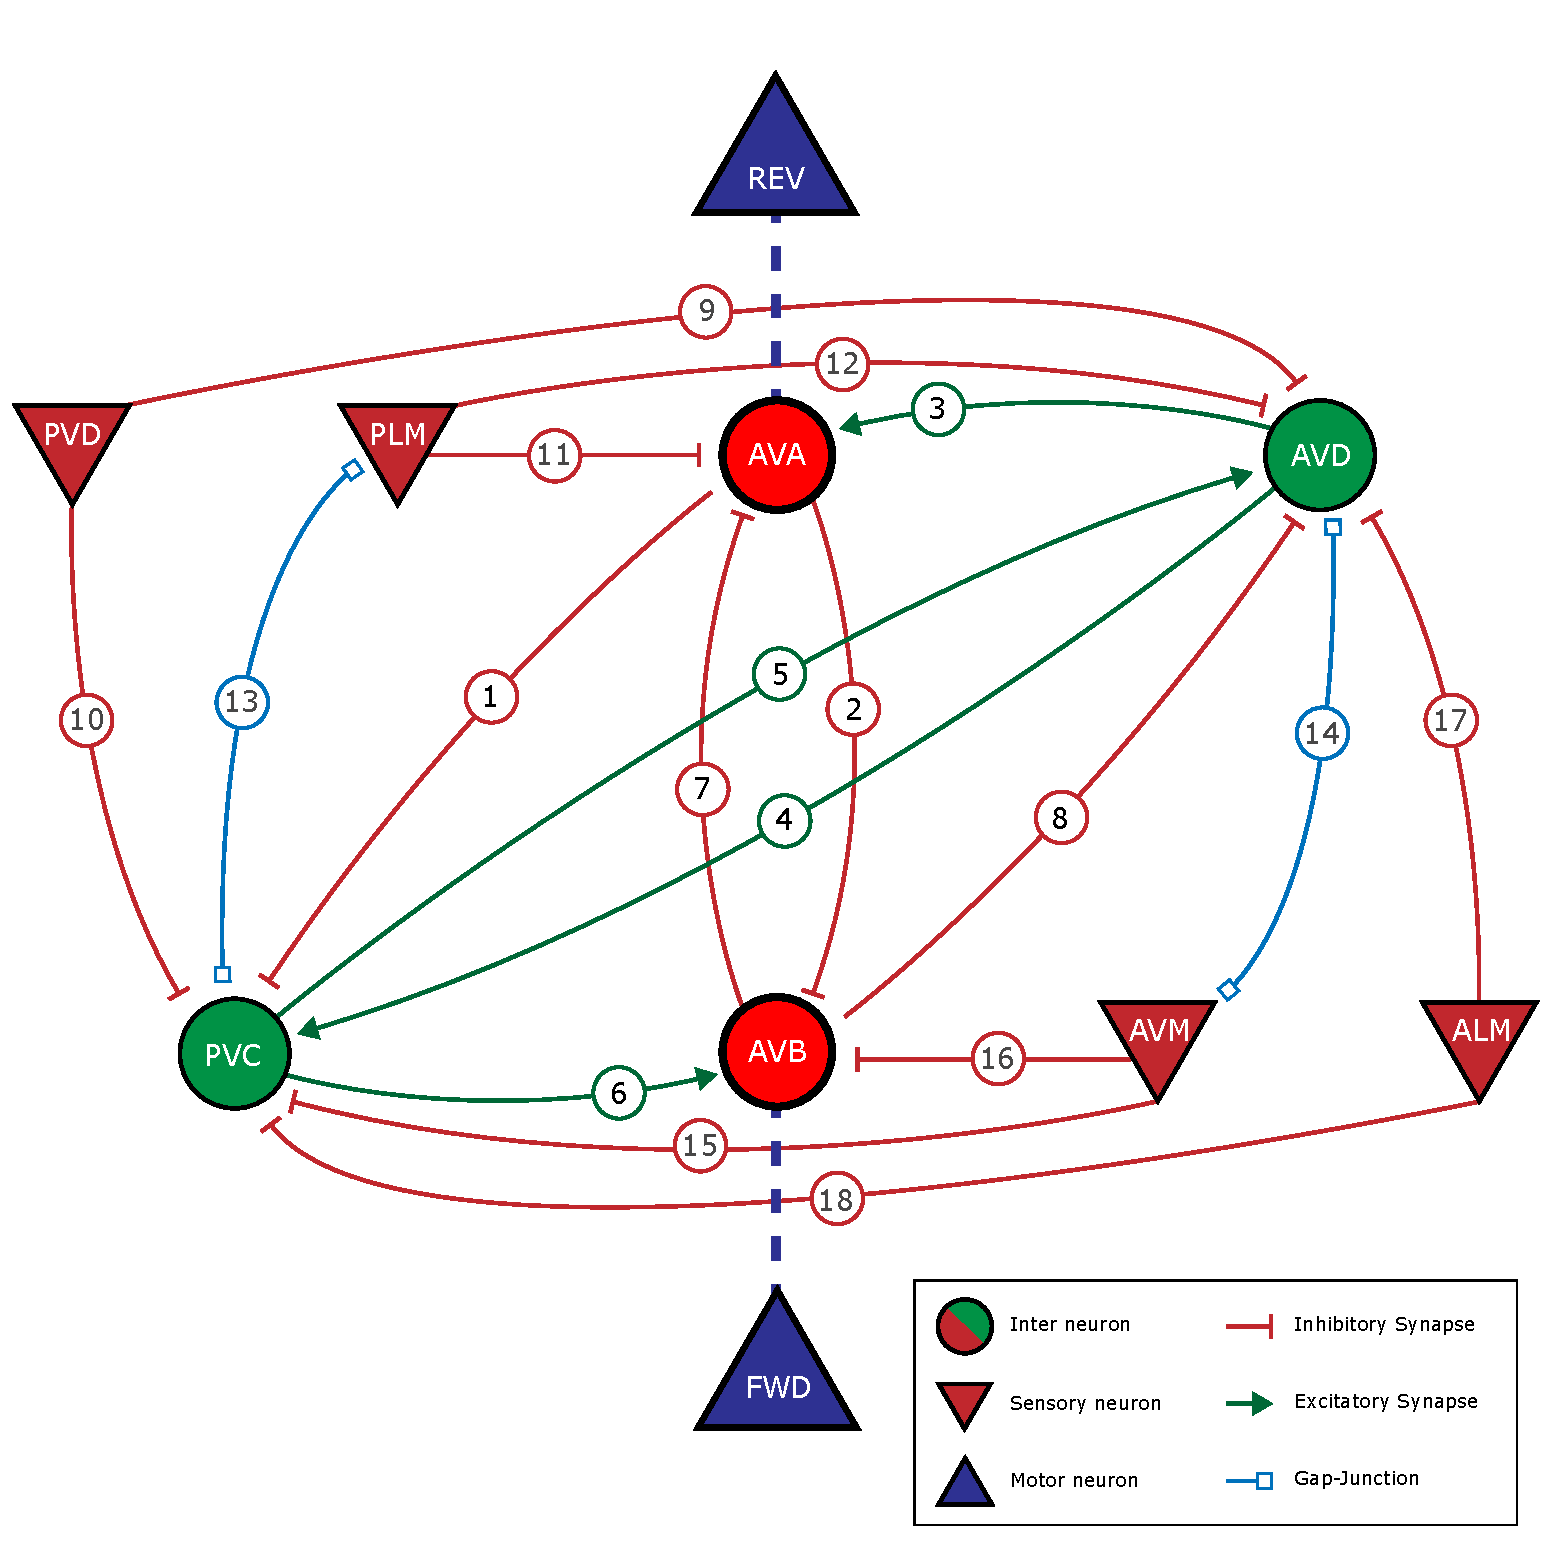
\includegraphics[width=12cm]{figures/appendix/Neural_Net_v3_num_syn.pdf}
		\caption{Neuronales Netz mit Legende für Gewichte.}
		\label{fig:erg_rs_flow}
	\end{figure}

	\afterpage{%
		\clearpage% Flush earlier floats (otherwise order might not be correct)
		\thispagestyle{empty}% empty page style (?)
		\begin{landscape}% Landscape page
			\centering % Center table
			\begin{tabular}{c@{\hskip 0.5cm}c@{\hskip 0.5cm}c@{\hskip 0.5cm}c@{\hskip 0.5cm}p{85mm}}    \toprule
				\setlength{\tabcolsep}{50pt}
				\renewcommand{\arraystretch}{1.5}
				\emph{Zeitstempel} 		& \emph{Algorithmus}		& \emph{Belohnung}	& \emph{Simulation (Dauer, Anz.)} 	& \emph{Parameter}		 \\\midrule
				
				20180817\_01-56-01		& \texttt{RandomSearch} - Parameter	& 131			& 12h, ca. 1 Mio. Simulationen		& Parameter der Nervenzellen \newline
				$\boldsymbol{C_m} = \begin{pmatrix}0.01, 0.01, 0.01, 0.01\end{pmatrix}$,\newline
				$\boldsymbol{G_{Leak}} = \begin{pmatrix}1.42, 0.63, 1.42, 0.63\end{pmatrix}$,\newline
				$\boldsymbol{U_{Leak}} = \begin{pmatrix}-63.2, -62.2, -63.2, -62.2\end{pmatrix}.$ \vspace{0.2cm} \newline
				Parameter der Synapsen \& Gap-Junctions \newline
				$\boldsymbol{\sigma} = \begin{pmatrix}0.16, 0.49, 0.15, 0.29, 0.16, 0.49, 0.15, 0.29,\\ 0.13, 0.39, 0.17, 0.06, 0.13, 0.39, 0.17, 0.06\end{pmatrix}$,\newline
				$\boldsymbol{w} = \begin{pmatrix}0.97, 1.57, 1.48, 1.28, 0.97, 1.57, 1.48, 1.28,\\ 1.71, 1.45, 0.78, 2.84, 1.71, 1.45, 0.78, 2.84\end{pmatrix}$,\newline
				$\boldsymbol{\hat{w}} = \begin{pmatrix}1.84, 1.84\end{pmatrix}$.\vspace{0.5cm}\\
				
				20180817\_13-56-01		& \texttt{Weights} - Gewichte		& 200			& 12h, ca. 400.000 Simulationen		& Gewichte der Synapsen \newline
				$\boldsymbol{g} = \begin{pmatrix}0.94, 0.96, 0.95, 0.14, 0.94, 0.96, 0.95, 0.14, 0.75,\\ 0.45, 0.54, 0.21, 0.97, 0.75, 0.45, 0.54, 0.21, 0.97\end{pmatrix}$.\vspace{0.5cm}\\
				
				20180905\_14-19-10		& \texttt{Genetic\_Algorithm} - Parameter& 200			& 1:30 Min, ca. 50 Tsd. Simulationen		& Parameter der Nervenzellen \newline
				$\boldsymbol{C_m} = \begin{pmatrix}0.04, 0.58, 0.58, 0.04\end{pmatrix}$,\newline
				$\boldsymbol{G_{Leak}} = \begin{pmatrix}0.75, 0.30, 0.30, 0.75\end{pmatrix}$,\newline
				$\boldsymbol{U_{Leak}} = \begin{pmatrix}-58.7, -55.6, -55.6, -58.7\end{pmatrix}.$ \vspace{0.2cm} \newline
				Parameter der Synapsen \& Gap-Junctions \newline
				$\boldsymbol{\sigma} = \begin{pmatrix}0.17, 0.37, 0.42, 0.15, 0,15 0.42, 0.37, 0.17,\\ 0.26, 0.27, 0.46, 0.20, 0.20, 0.46, 0.27, 0.26\end{pmatrix}$,\newline
				$\boldsymbol{w} = \begin{pmatrix}0.31, 0.18, 2.45, 0.93, 0,93 2.45, 0.18, 0.31,\\ 0.97, 1.21, 1.25, 0.53, 0.53, 1.25, 1.21, 0.97\end{pmatrix}$,\newline
				$\boldsymbol{\hat{w}} = \begin{pmatrix}2.40, 2.40\end{pmatrix}$.\vspace{0.5cm}\\
				
				\bottomrule
				\hline
			\end{tabular}
			\captionof{table}{Simulationsläufe mit guten Ergebnissen}% Add 'table' caption
			\label{tab:app_erg}
		\end{landscape}
		\clearpage% Flush page
	}
	


%%% Local Variables: 
%%% mode: latex
%%% TeX-master: "main"
%%% End: 
